\section{Vista general}
En esta sección se tratan los aspectos relacionados con la con la implementación
del sistema y su codificación. Para ello se describen las herramientas software
y hardware utilizadas en el desarrollo, y la estructra del código fuente. 

\section{Entorno de construcción}

\begin{description}
   \item[Entodrno de desarrollo (IDE):] Geany
   \item[Lenguaje de programación:] C++
   \item[Compilador:] GCC
   \item[Configuración automática:] Autoconf
   \item[Construcción automática:] Automake
   \item[Gestión de dependencias:] Make
   \item[Control de versions:] Subversion
   \item[Generador de analizador léxico:] Flex
   \item[Generador de analizador sintáctico:] Bison
   \item[Depurador:] GDB
   \item[Bibliotecas de desarrollo] \hfill 
      \begin{description}
         \item[Editor de línea e histórico:] Readline
         \item[Expresiones regulares:] BoostRegex
         \item[Matemáticas:] Biblioteca estándar de C
         \item[Enlaces dinámicos:] Biblioteca del sistema GNU/Linux libdl
      \end{description}
   \item[Desarrollo Web] \hfill 
      \begin{description}
         \item[Programación en servidor:] PHP
         \item[Programación en cliente:] JavaScript
         \item[Estructura del contenido:] HTML5
         \item[Presentación del contenido:] CSS
      \end{description}
\end{description}

\section{Ficheros de código fuente}
El sistema software se constituye de una serie de módulos o componentes en forma de ficheros, 
cada uno de los cuales contine las estructuras de programación y el código fuente necesario
para implementar cada una de las funcionalidades del sistema.

\begin{description}
\item [interpreter:] Interprete.
\item [lshScanner:] Analizador léxico.
\item [lshParser:] Analizador sintáctico.
\item [error:] Sistema de errores.
\item [plugins:] Sistema de extensiones.
\item [run/runTree:] Abstracción de nodo ejecutable.
\item [run/expNode:] Abstracción de nodos ejecutables expresiones.
\item [run/symbols:] Estructura de datos tabla de símbolos.
\item [run/sTable:] Gestión de tabla de de símbolos y definiciones.
\item [run/typeNode:] Nodos ejecutables para cada tipo de dato.
\item [run/numData:] Representación interna de datos numéricos.
\item [run/stmtNode:] Nodos ejecutables sentencias de control.
\item [run/operatorBaseNode:] Nodos ejecutables operadores básicos.
\item [run/operatorLogicNode:] Nodos ejecutables operadores lógicos.
\item [run/operatorArithNode:] Nodos ejecutables operadores aritméticos.
\item [run/operatorStrNode:] Nodos ejecutables operadores sobre cadenas.
\item [run/operatorArrayNode:] Nodos ejecutables operadores sobre arrays.
\item [run/operatorRegexpNode:] Nodos ejecutables operadores sobre expresiones regulares.
\item [run/operatorDateNode:] Nodos ejecutables operadores sobre fechas y tiempo.
\item [run/operatorFileNode:] Nodos ejecutables operadores sobre ficheros.
\item [run/operatorProcessNode:] Nodos ejecutables operadores sobre procesos.
\end{description}

A continuación se describen las dependencias entre ficheros mediante una serie de paquetes que contienen diagramas de componentes.
Este aspecto del sistema queda completamente descrito mediante la combinación de estos paquetes.

\begin{center}
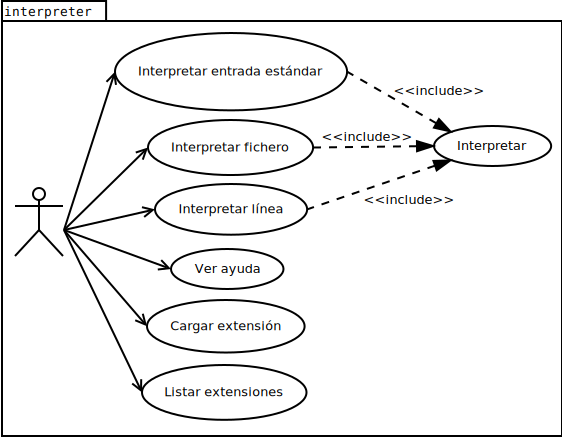
\includegraphics[scale=0.3]{files_arquitecture/interpreter.png} \\
\end{center}
\pagebreak
\begin{multicols}{2}
\begin{center}
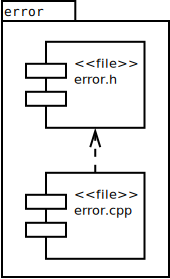
\includegraphics[scale=0.3]{files_arquitecture/error.png} \\
\end{center}
\begin{center}
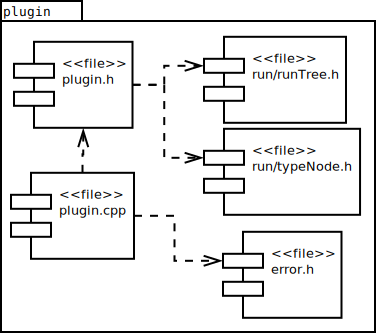
\includegraphics[scale=0.3]{files_arquitecture/plugin.png} \\
\end{center}
\end{multicols}

\begin{multicols}{2}
\begin{center}
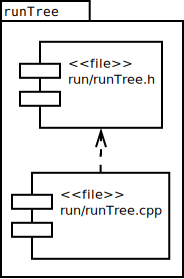
\includegraphics[scale=0.3]{files_arquitecture/runTree.png} \\
\end{center}
\begin{center}
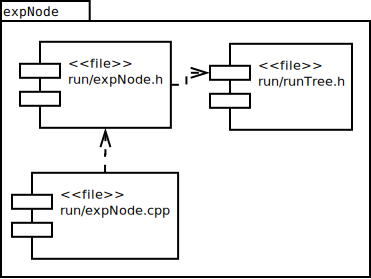
\includegraphics[scale=0.3]{files_arquitecture/expNode.png} \\
\end{center}
\end{multicols}

\begin{multicols}{2}
\begin{center}
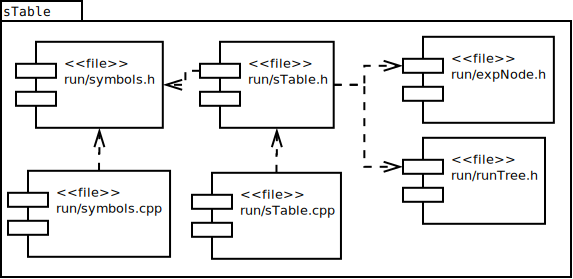
\includegraphics[scale=0.3]{files_arquitecture/sTable.png} \\
\end{center}
\begin{center}
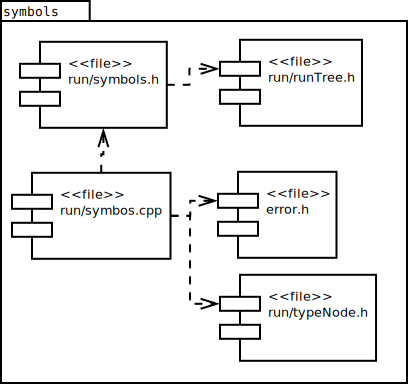
\includegraphics[scale=0.3]{files_arquitecture/symbols.png} \\
\end{center}
\end{multicols}

\begin{multicols}{2}
\begin{center}
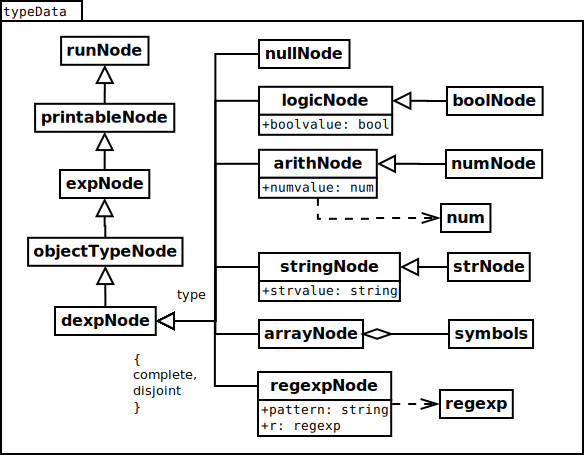
\includegraphics[scale=0.3]{files_arquitecture/typeData.png} \\
\end{center}
\begin{center}
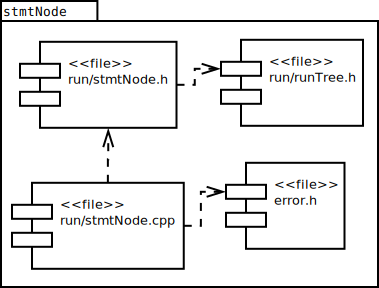
\includegraphics[scale=0.3]{files_arquitecture/stmtNode.png} \\
\end{center}
\end{multicols}
\pagebreak
\begin{multicols}{2}
\begin{center}
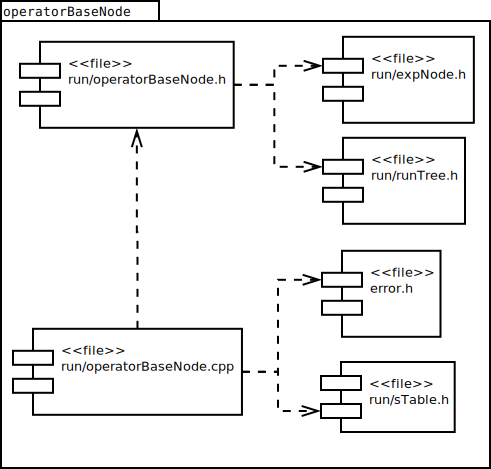
\includegraphics[scale=0.3]{files_arquitecture/operatorBaseNode.png} \\
\end{center}
\begin{center}
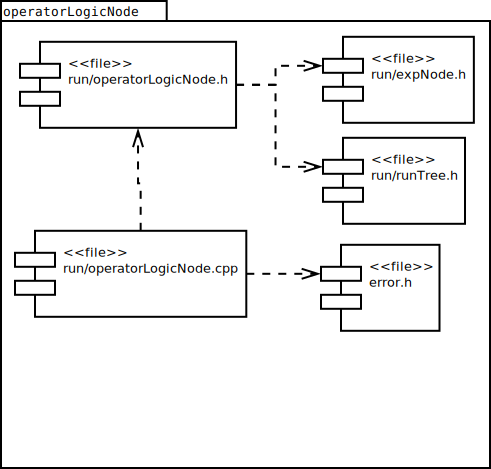
\includegraphics[scale=0.3]{files_arquitecture/operatorLogicNode.png} \\
\end{center}
\end{multicols}

\begin{multicols}{2}
\begin{center}
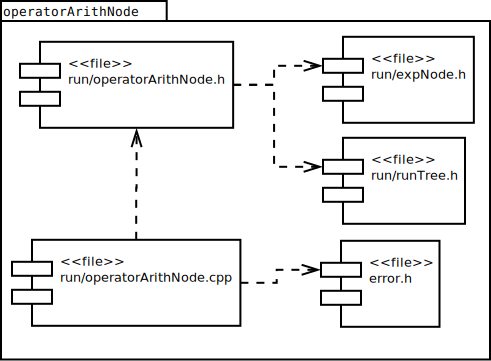
\includegraphics[scale=0.3]{files_arquitecture/operatorArithNode.png} \\
\end{center}
\begin{center}
\includegraphics[scale=0.3]{files_arquitecture/operatorStrNode.png} \\
\end{center}
\end{multicols}


\begin{multicols}{2}
\begin{center}
\includegraphics[scale=0.3]{files_arquitecture/operatorArrayNode.png} \\
\end{center}
\begin{center}
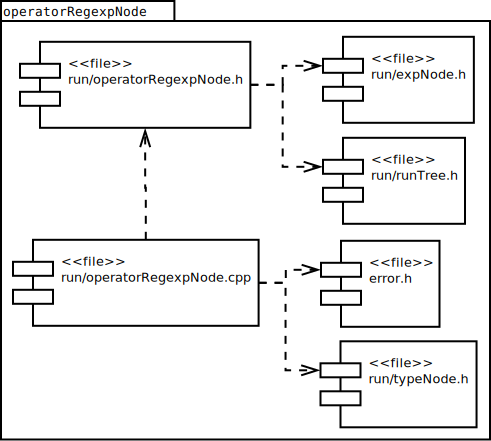
\includegraphics[scale=0.3]{files_arquitecture/operatorRegexpNode.png} \\
\end{center}
\end{multicols}

\begin{multicols}{2}
\begin{center}
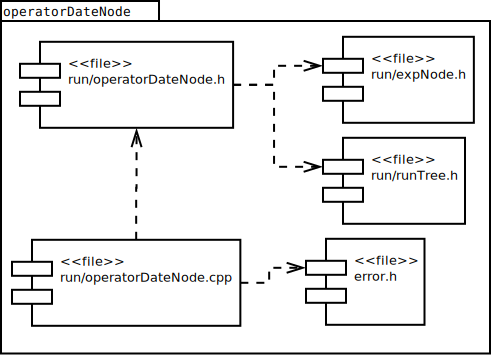
\includegraphics[scale=0.3]{files_arquitecture/operatorDateNode.png} \\
\end{center}
\begin{center}
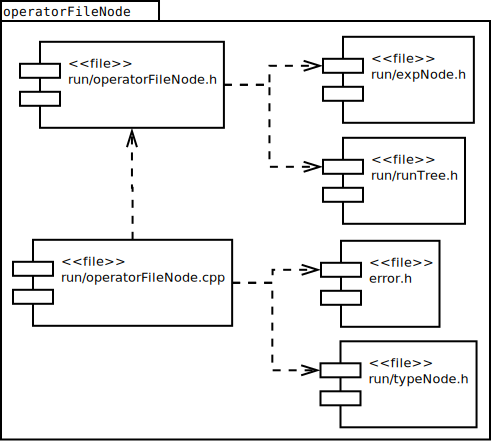
\includegraphics[scale=0.3]{files_arquitecture/operatorFileNode.png} \\
\end{center}
\end{multicols}


%~ \begin{multicols}{2}
\begin{center}
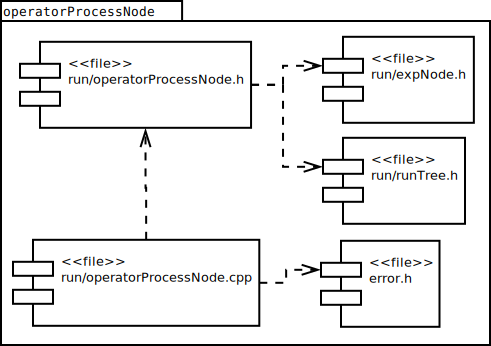
\includegraphics[scale=0.3]{files_arquitecture/operatorProcessNode.png} \\
\end{center}
%~ \end{multicols}

